% Enable warnings about problematic code
\RequirePackage[l2tabu, orthodox]{nag}

\documentclass{WeSTassignment}

% The lecture title, e.g. "Web Information Retrieval".
\lecture{Introduction to Web Science}
% The names of the lecturer and the instructor(s)
\author{%
  Prof. Dr.~Steffen~Staab\\{\normalsize\mailto{staab@uni-koblenz.de}} \and
  Ren{\'e}~Pickhardt\\{\normalsize\mailto{rpickhardt@uni-koblenz.de}} \and
   Korok~Sengupta\\{\normalsize\mailto{koroksengupta@uni-koblenz.de}}
}
% Assignment number.
\assignmentnumber{2}
% Institute of lecture.
\institute{%
  Institute of Web Science and Technologies\\%
  Department of Computer Science\\%
  University of Koblenz-Landau%
}
% Date until students should submit their solutions.
\datesubmission{November 9, 2016, 10:00 a.m.}
% Date on which the assignments will be discussed in the tutorial.
\datetutorial{November 11th, 2016, 12:00 p.m.}

% Set langauge of text.
\setdefaultlanguage[
  variant = american, % Use American instead of Britsh English.
]{english}

% Specify bib file location.
\addbibresource{bibliography.bib}

% For left aligned centerd boxes
% see http://tex.stackexchange.com/a/25591/75225
\usepackage{varwidth}

% ==============================================================================
% Document

\begin{document}

\maketitle

The main objective of this assignment is for you to use different tools with which you can understand the network that you are connected to or you are connecting to in a better sense.
These tasks are not always specific to \enquote{Introduction to Web Science}.
For all the assignment questions that require you to write a code, make sure to include the code in the answer sheet, along with a separate python file. Where screen shots are required, please add them in the answers directly and not as separate files. 
\\
\\
\\
\\ 
{\Large Group name: echo\par} \\
{\Large Group Member: Hanadi Tamimi, Keya Kashem, Md Jakaria Nawaz\par} \\

% ------------------------------------------------------------------------------

\section{IP Packet (5 Points)}

Consider the IPv4 packet that is received as:\\ \\
\texttt{4500 062A 42A1 8001 4210 XXXX C0A8 0001 C0A8 0003}\\ \\ 
Consider \texttt{XXXX} to be the check sum field that needs to be sent with the packet.

Please provide a step-by-step process for calculating the "Check Sum".\\ \\ 

%Answer
\underline{Answers:}

\begin{enumerate}
Getting sum of all bits except checksum bits\\
4500 + 062A + 42A1 + 8001 + 4210 + C0A8 + 0001 + C0A8 + 0003 = 2 D130 \\
Binary value of 2 D130 = 0010 1101 0001 0011 0000 \\ \\
There has to be 16 bits value. So, we need to add first 4 bits with the rest of the value as carry:\\
0010 + 1101 0001 0011 0000 = 1101 0001 0011 0010 \\ \\
Complement of the 16 bit value: 0010 1110 1100 1101 \\
Hexadecimal equivalent of 0010 1110 1100 1101 = 2ECD (Check Sum)\\

\end{enumerate}



% ------------------------------------------------------------------------------

\section{Routing Algorithm (10 Points)}
You have seen how routing tables can be used to see how the packets are transferred across different networks. Using the routing tables below of Router 1, 2 and 3:
\begin{enumerate}
\item Draw the network \texttt{[6 points]}
\item Find the shortest path of sending information from 67.68.2.10 network to 25.30.3.13 network \texttt{[4 points]}
\end{enumerate}

\begin{table}[h]
\centering
\caption{Router 1}
\label{Router 1}
\begin{tabular}{ccc}
\hline
\multicolumn{1}{|c|}{\textbf{Destination}} & \multicolumn{1}{c|}{\textbf{Next Hop}} & \multicolumn{1}{c|}{\textbf{Interface}} \\ \hline
67.0.0.0                                   & 67.68.3.1                              & eth 0                                   \\
62.0.0.0                                   & 62.4.31.7                              & eth 1                                   \\
88.0.0.0                                   & 88.4.32.6                              & eth 2                                    \\
141.0.0.0                                  & 141.30.20.1                            & eth 3                                    \\
26.0.0.0                                   & 141.71.26.3                            & eth 3                                   \\
150.0.0.0                                  & 141.71.26.3                            & eth 3                                   \\
205.0.0.0                                  & 141.71.26.3                            & eth 3                                    \\
25.0.0.0                                   & 88.6.32.1                              & eth 2                                    \\
121.0.0.0                                  & 88.6.32.1                              & eth 2                                   
\end{tabular}
\end{table}
\begin{table}[h]
\centering
\caption{Router 2}
\label{Router 2}
\begin{tabular}{ccc}
\hline
\multicolumn{1}{|c|}{\textbf{Destination}} & \multicolumn{1}{c|}{\textbf{Next Hop}} & \multicolumn{1}{c|}{\textbf{Interface}} \\ \hline
141.0.0.0                                  & 141.71.26.3                            & eth 3                                   \\
205.0.0.0                                  & 205.25.71.1                            & eth 0                                   \\
26.0.0.0                                   & 26.3.2.1                               & eth 2                                    \\
156.0.0.0                                  & 156.3.0.6                              & eth 1                                   \\
67.0.0.0                                   & 141.30.20.1                            & eth 3                                   \\
62.0.0.0                                   & 141.30.20.1                            & eth 3                                   \\
88.0.0.0                                   & 141.30.20.1                            & eth 3                                    \\
25.0.0.0                                   & 205.30.7.2                             & eth 0                                   \\
121.0.0.0                                  & 205.30.7.2                             & eth 0                                  
\end{tabular}
\end{table}
\begin{table}[h]
\centering
\caption{Router 3}
\label{Router 3}
\begin{tabular}{ccc}
\hline
\multicolumn{1}{|c|}{\textbf{Destination}} & \multicolumn{1}{c|}{\textbf{Next Hop}} & \multicolumn{1}{c|}{\textbf{Interface}} \\ \hline
205.0.0.0                                  & 205.30.7.2                             & eth 0                                   \\
88.0.0.0                                   & 88.6.32.1                              & eth 1                                   \\
25.0.0.0                                   & 25.30.1.2                              & eth 2                                   \\
121.0.0.0                                  & 121.0.3.1                              & eth 3                                   \\
156.0.0.0                                  & 205.25.7.1                             & eth 0                                   \\
26.0.0.0                                   & 205.25.7.1                             & eth 0                                   \\
141.0.0.0                                  & 205.25.7.1                             & eth 0                                   \\
67.0.0.0                                   & 88.4.32.6                              & eth 1                                   \\
62.0.0.0                                   & 88.4.32.6                              & eth 1                                  
\end{tabular}
\end{table} \\

(1)\\
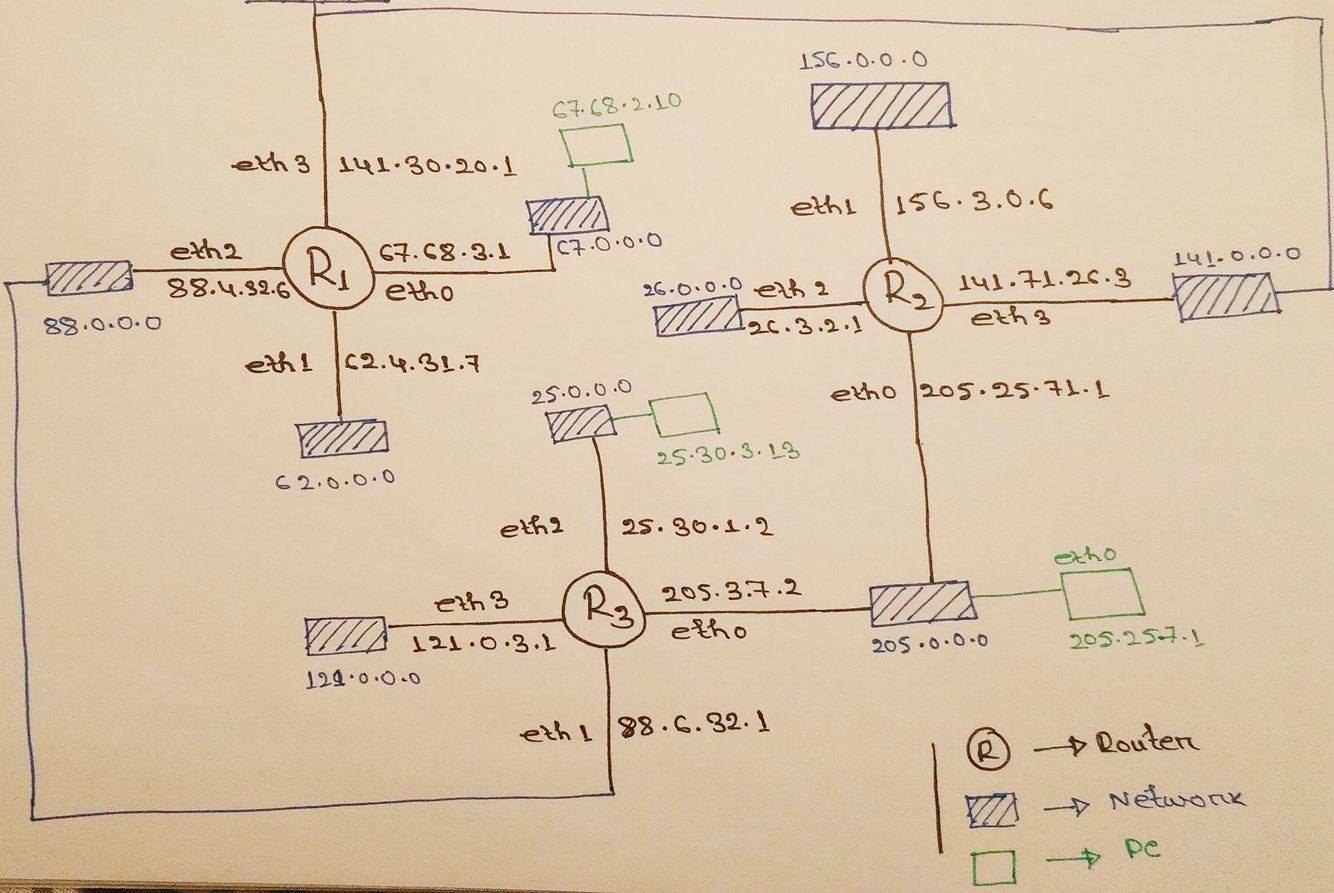
\includegraphics[width=1\textwidth]{images/route_table_1.jpg} \\
According to the first given routing table. NOT according to the updated question.\\
(2)\\
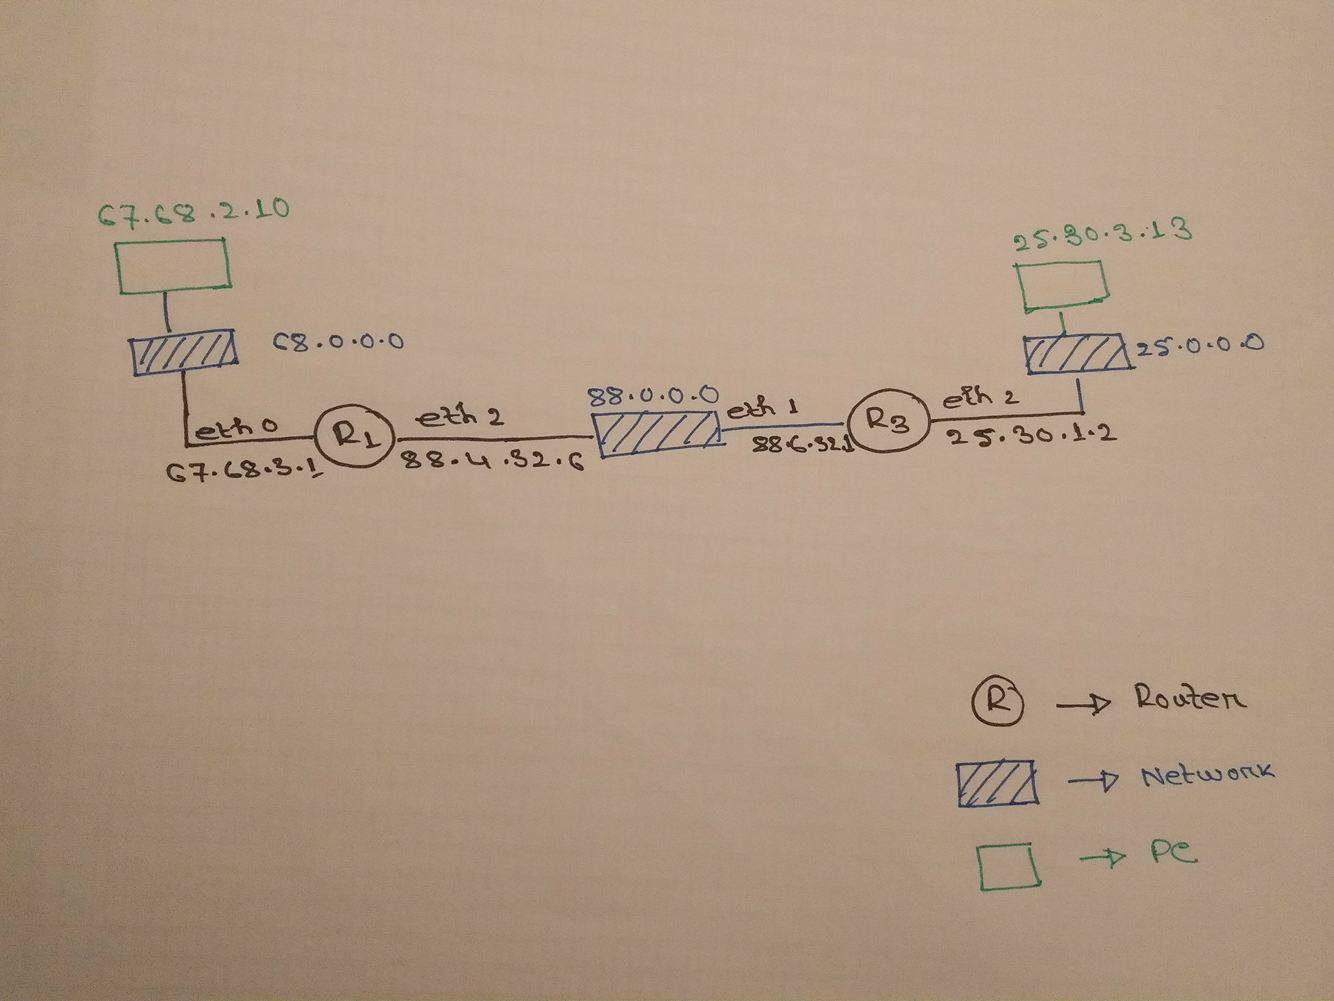
\includegraphics[width=1\textwidth]{images/route_table_2.jpg} \\ \\
According to the first given routing table. NOT according to the updated question.\\
% ------------------------------------------------------------------------------
\section{Sliding Window Protocol (10 Points)}
\emph{Sliding window algorithm, which allows a sender to have more than one unacknowledged packet "in flight" at a time, improves network throughput. }\\ \\
Let us consider you have 2 Wide Area Networks. One with a bandwidth of 10 Mbps (Delay of 20 ms) and the other with 1 Mbps (Delay of 30 ms) . If a packet is considered to be of size 10kb. Calculate the window size of number of packets necessary for Sliding Window Protocol. [\texttt{5 points}]\\ \\
Since you now understand the concept of Window Size for Sliding Window Protocol and how to calculate it, consider a window size of 3 packets and you have 7 packets to send. Draw the process of \texttt{Selective Repeat Sliding Window Protocol} where in the 3rd packet from the sender is lost while transmission. Show diagrammatically how the system reacts when a packet is not received and how it recuperates from that scenario. [\texttt{5 points}] \\

\underline{Answer:}

1. Calculation:  \\
WAN 1 \\
In 10$\string^$3 ms it transmits (8 * 10 * 10$\string^$6 ) bits \\
In 20 ms it transmits X bits \\
X = (8 * 10 * 10$\string^$6 ) bits * 20 ms / 10$\string^$3 ms = 160 * 10$\string^$4 bits \\
So, 1 frame is of 10 kb or 80000 bits \\
So total number of frames,\\
= 160 * 10$\string^$4 bits \ 80000 bits = 20 [Window Size] \\ \\

WAN 2 \\ 
In 10$\string^$3 ms it transmits (8 * 10$\string^$6 ) bits \\
In 30 ms it transmits X bits \\
X = (8 * 10$\string^$6 ) bits * 30 ms / 10$\string^$3 ms = 240 * 10$\string^$3 bits \\
So, 1 frame is of 10 kb or 80000 bits \\
So total number of frames,\\
= 240 * 10$\string^$3 bits \ 80000 bits = 3 [Window Size] \\

2. Diagram: \\
\includegraphics[scale=.5]{images/packet_send_ack.png} \\

In selective repeat sliding window protocol the packets don't have to be sent sequentially that means if the acknowledgement of any packets not received, next packet will be transmitted and after the time period of time out session the missing packet will be transmitted. It does not have to be like p0, p1, p2, p3 and so on, it can be p0,p1,p3,p4,p2 and so on.
% ------------------------------------------------------------------------------

\section{TCP Client Server (10 Points)}

Use the information from the \href{https://docs.python.org/3/howto/sockets.html}{socket} documentation and create: [\texttt{4 points}]
\begin{enumerate}
\item a simple TCP Server that listens to a
\item Client
\end{enumerate}
\underline{Note:} Please use port \texttt{8080} for communication on \texttt{localhost} for client server communication.\\ \\
Given below are the following points that your client and server must perform: [\texttt{6 points}]
\begin{enumerate}
\item The \emph{Client} side asks the user to input their name, age \& \emph{matrikelnummer} which is then sent to the server all together.
\item Develop a protocol for sending these three information and subsequently receiving each of the information in three different lines as mentioned in the below format. Provide reasons for the protocol you implemented. 
\item Format the output in a readable format as:\texttt{\\ Name: Korok Sengupta; \\ Age: 29; \\ Matrikelnummer: 21223ert56}
\end{enumerate}

Provide a snapshot of the results along with the code. \\

\underline{Answer:} \\
Code: \\
Client: \\
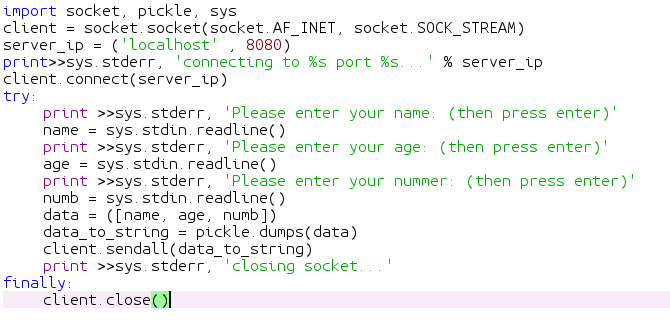
\includegraphics[width=1\textwidth]{images/code1.png} \\ \\
Server: \\
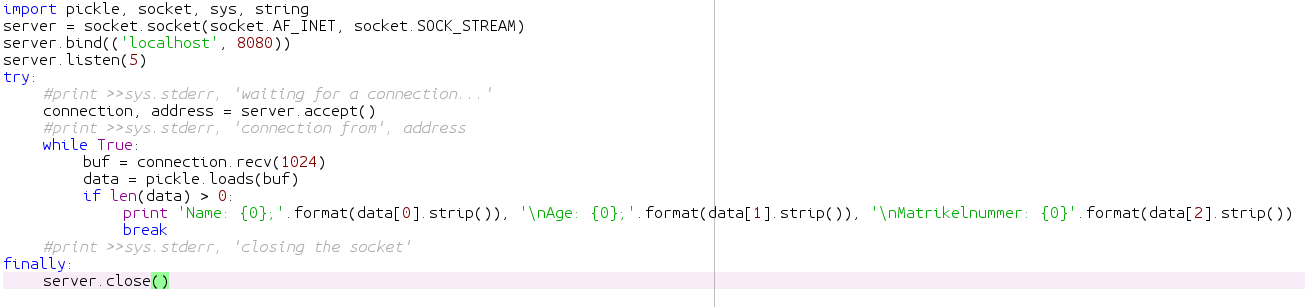
\includegraphics[width=1\textwidth]{images/code2_server.png} \\ \\
Output Image: \\
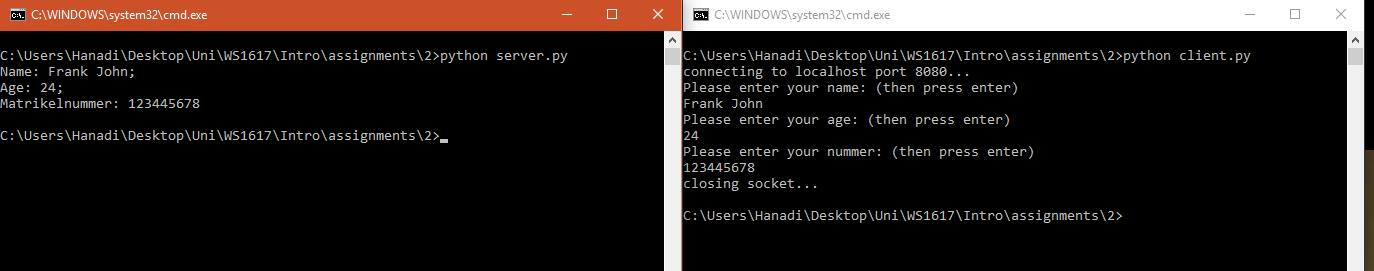
\includegraphics[width=1\textwidth]{images/output_pic.png} \\ \\

\makefooter

\end{document}
